% Digital Logic Report Template
% Created: 2020-01-16 Sebastian Lopez 

%==========================================================
%=========== Document Setup  ==============================

% Formatting defined by class file
\documentclass[11pt]{article}

% ---- Document formatting ----
\usepackage[margin=1in]{geometry}	% Narrower margins
\usepackage{booktabs}				% Nice formatting of tables
\usepackage{graphicx}				% Ability to include graphics

%\setlength\parindent{0pt}	% Do not indent first line of paragraphs 
\usepackage[parfill]{parskip}		% Line space b/w paragraphs
%	parfill option prevents last line of pgrph from being fully justified

% Parskip package adds too much space around titles, fix with this
\RequirePackage{titlesec}
\titlespacing\section{0pt}{8pt plus 4pt minus 2pt}{3pt plus 2pt minus 2pt}
\titlespacing\subsection{0pt}{4pt plus 4pt minus 2pt}{-2pt plus 2pt minus 2pt}
\titlespacing\subsubsection{0pt}{2pt plus 4pt minus 2pt}{-6pt plus 2pt minus 2pt}

% ---- Hyperlinks ----
\usepackage[colorlinks=true,urlcolor=blue]{hyperref}	% For URL's. Automatically links internal references.

% ---- Code listings ----
\usepackage{listings} 					% Nice code layout and inclusion
\usepackage[usenames,dvipsnames]{xcolor}	% Colors (needs to be defined before using colors)

% Define custom colors for listings
\definecolor{listinggray}{gray}{0.98}		% Listings background color
\definecolor{rulegray}{gray}{0.7}			% Listings rule/frame color

% Style for Verilog
\lstdefinestyle{Verilog}{
	language=Verilog,					% Verilog
	backgroundcolor=\color{listinggray},	% light gray background
	rulecolor=\color{blue}, 			% blue frame lines
	frame=tb,							% lines above & below
	linewidth=\columnwidth, 			% set line width
	basicstyle=\small\ttfamily,	% basic font style that is used for the code	
	breaklines=true, 					% allow breaking across columns/pages
	tabsize=3,							% set tab size
	commentstyle=\color{gray},	% comments in italic 
	stringstyle=\upshape,				% strings are printed in normal font
	showspaces=false,					% don't underscore spaces
}

% How to use: \Verilog[listing_options]{file}
\newcommand{\Verilog}[2][]{%
	\lstinputlisting[style=Verilog,#1]{#2}
}




%======================================================
%=========== Body  ====================================
\begin{document}

\title{ELC 2137 Lab \#3: Adders}
\author{Sebastian Lopez and Megan Gordon}

\maketitle


\section*{Summary}

In this lab we developed circuits that implement a given logic function, described the operation of half, full, and ripple adders, and we developed a moderately complex circuit on a breadboard using standard electrical parts. We also tested and verified the operation of each circuit. 

\section*{Q\&A}

\begin{table}[ht]\centering
	\caption{Half Adder Truth Table}
	\label{tbl:Logic_Truth_Table}
	\begin{tabular}{cc||cc||c}
		\toprule
		A & B & C & S & Decimal\\
		\midrule
		0 & 0 & 0 & 0 & 0\\
		0 & 1 & 0 & 1 & 1\\
		1 & 0 & 0 & 1 & 1\\
		1 & 1 & 1 & 0 & 2\\
		\bottomrule
	\end{tabular} 
\end{table} 

\begin{enumerate}
	\item Which gates could we use for combining the carry bits? 
	\item Which one should we use and why? 
\end{enumerate}

\section*{Results}

\begin{figure}[ht]\centering
	\includegraphics[width=0.75\textwidth, angle = 270]{Circuit Demonstration Page }
	\caption{This is the Circuit Demonstration Page.}
	\label{fig:original_logo}			% label must be after caption
\end{figure}

\begin{figure}[ht]\centering
	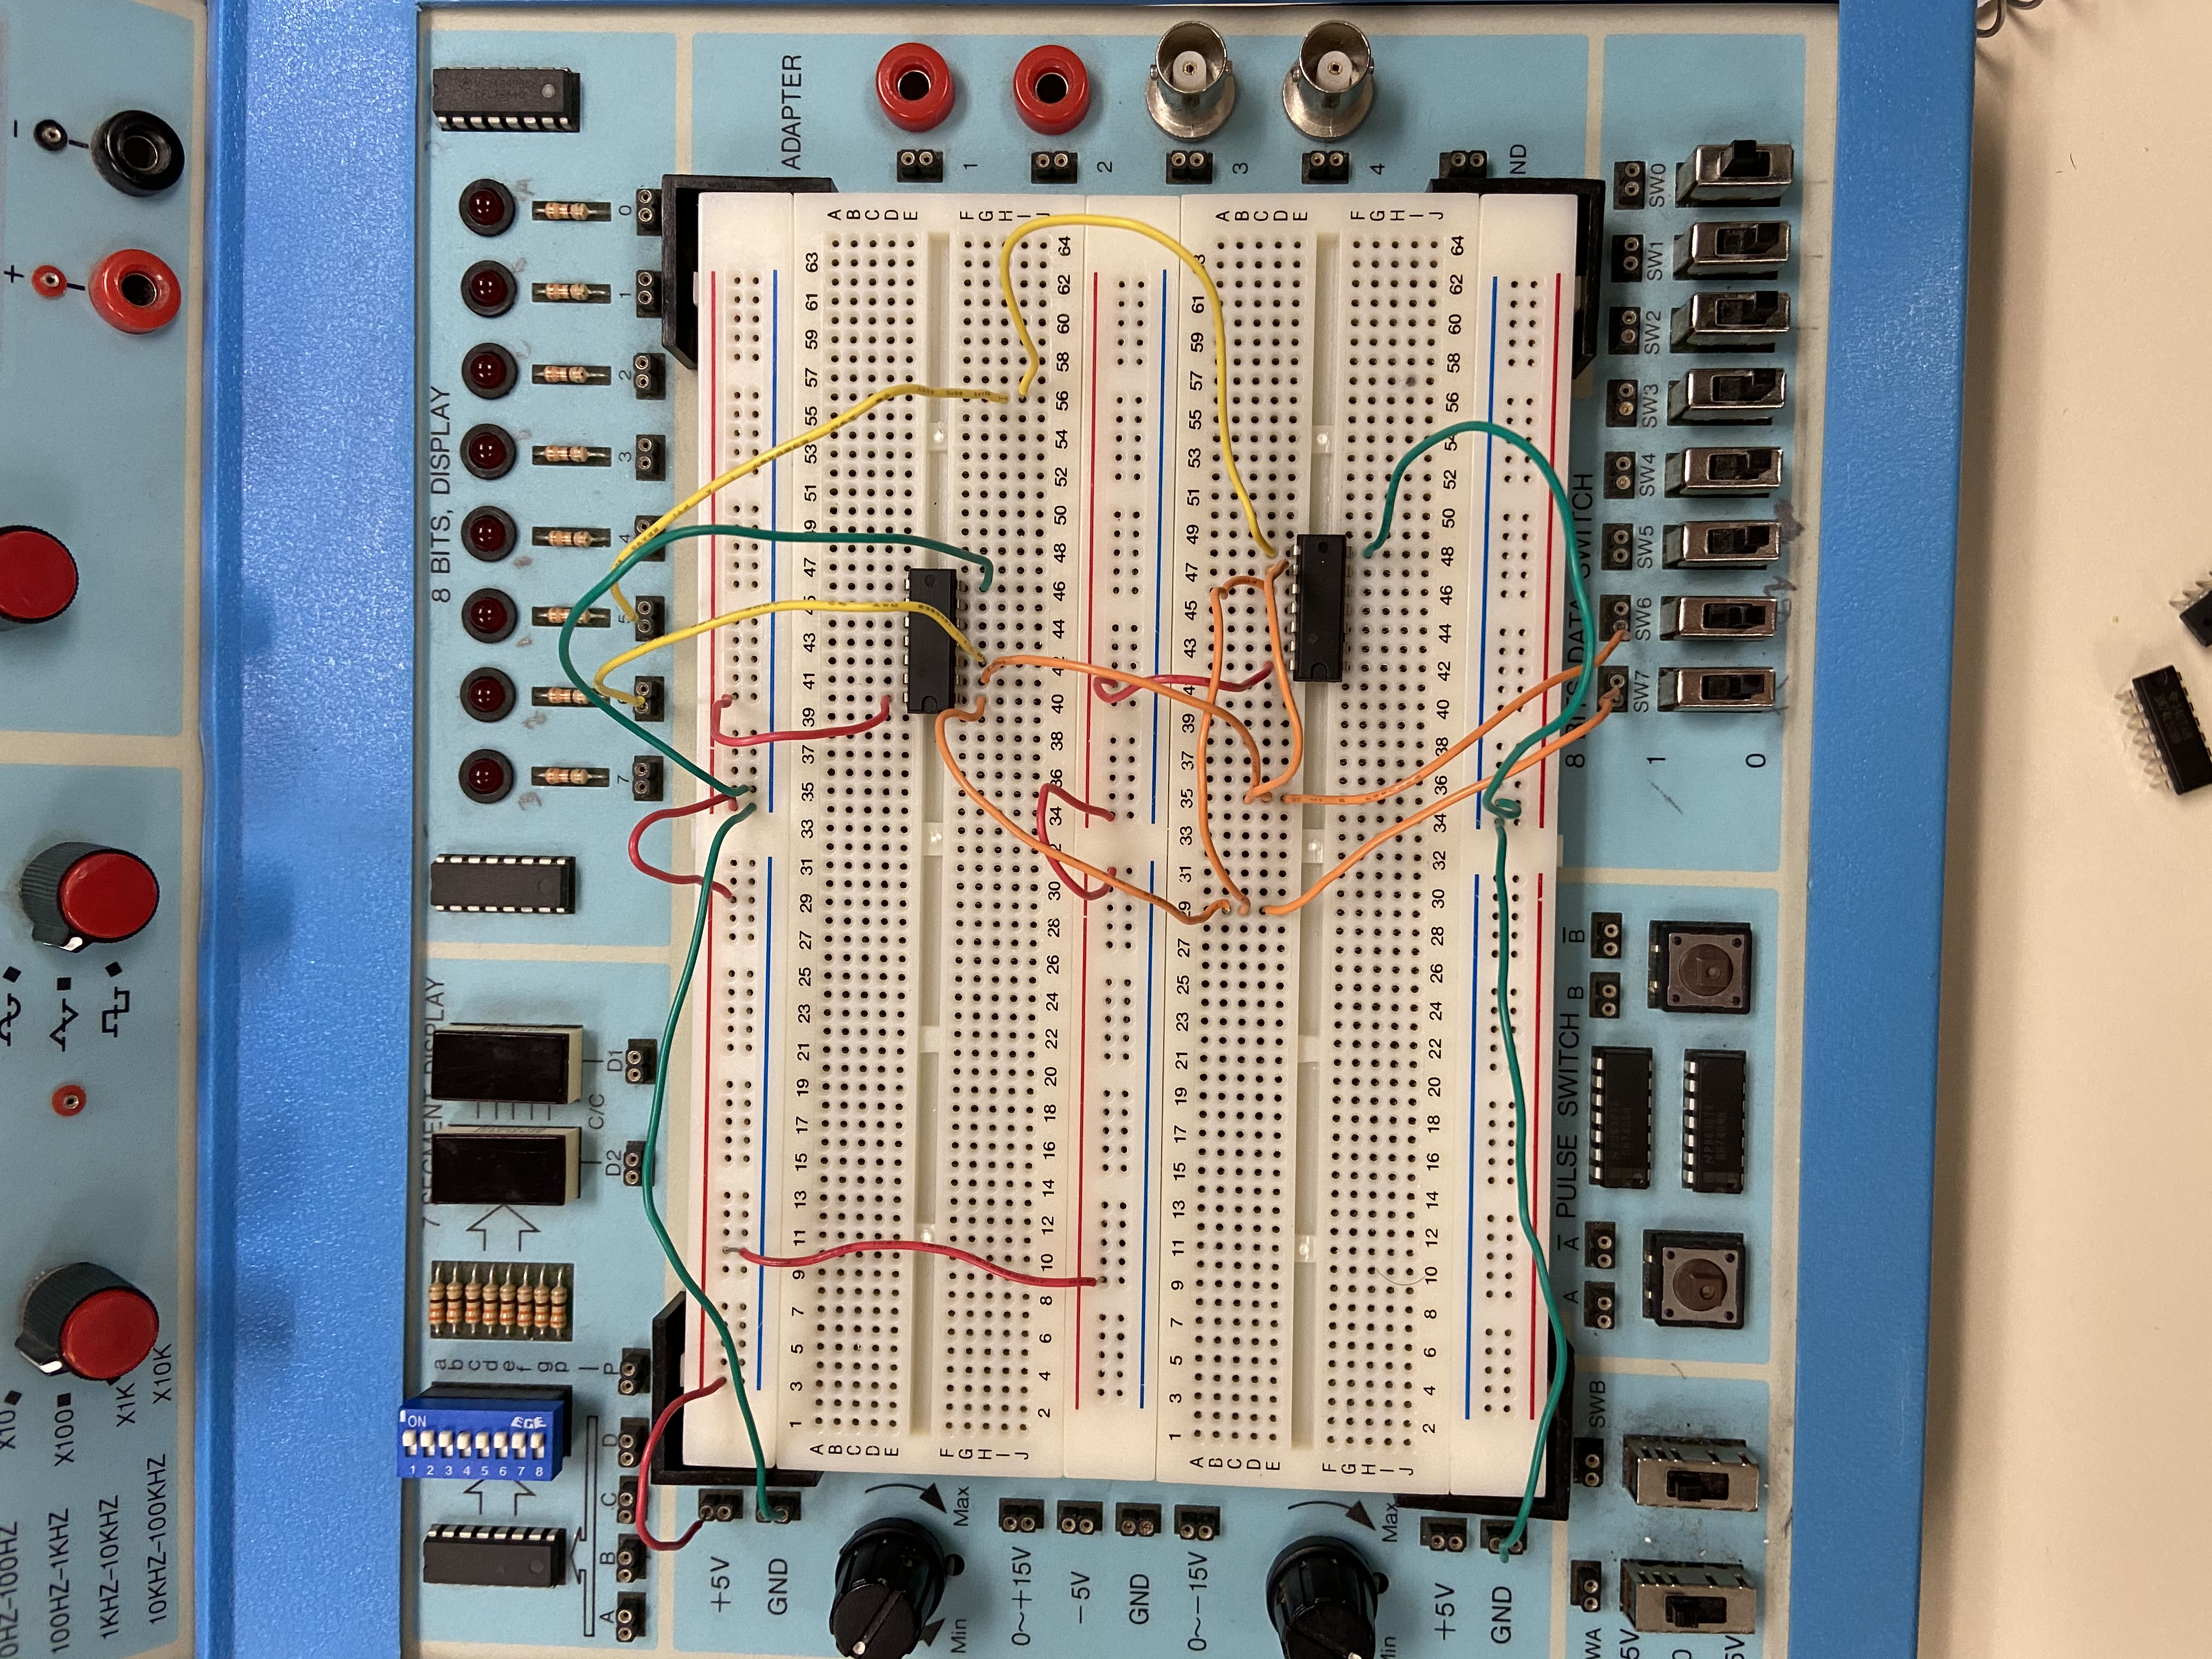
\includegraphics[width=0.75\textwidth, angle = 270]{Half Adder}
	\caption{This is the Half Adder.}
	\label{fig:original_logo}			% label must be after caption
\end{figure}

\begin{figure}[ht]\centering
	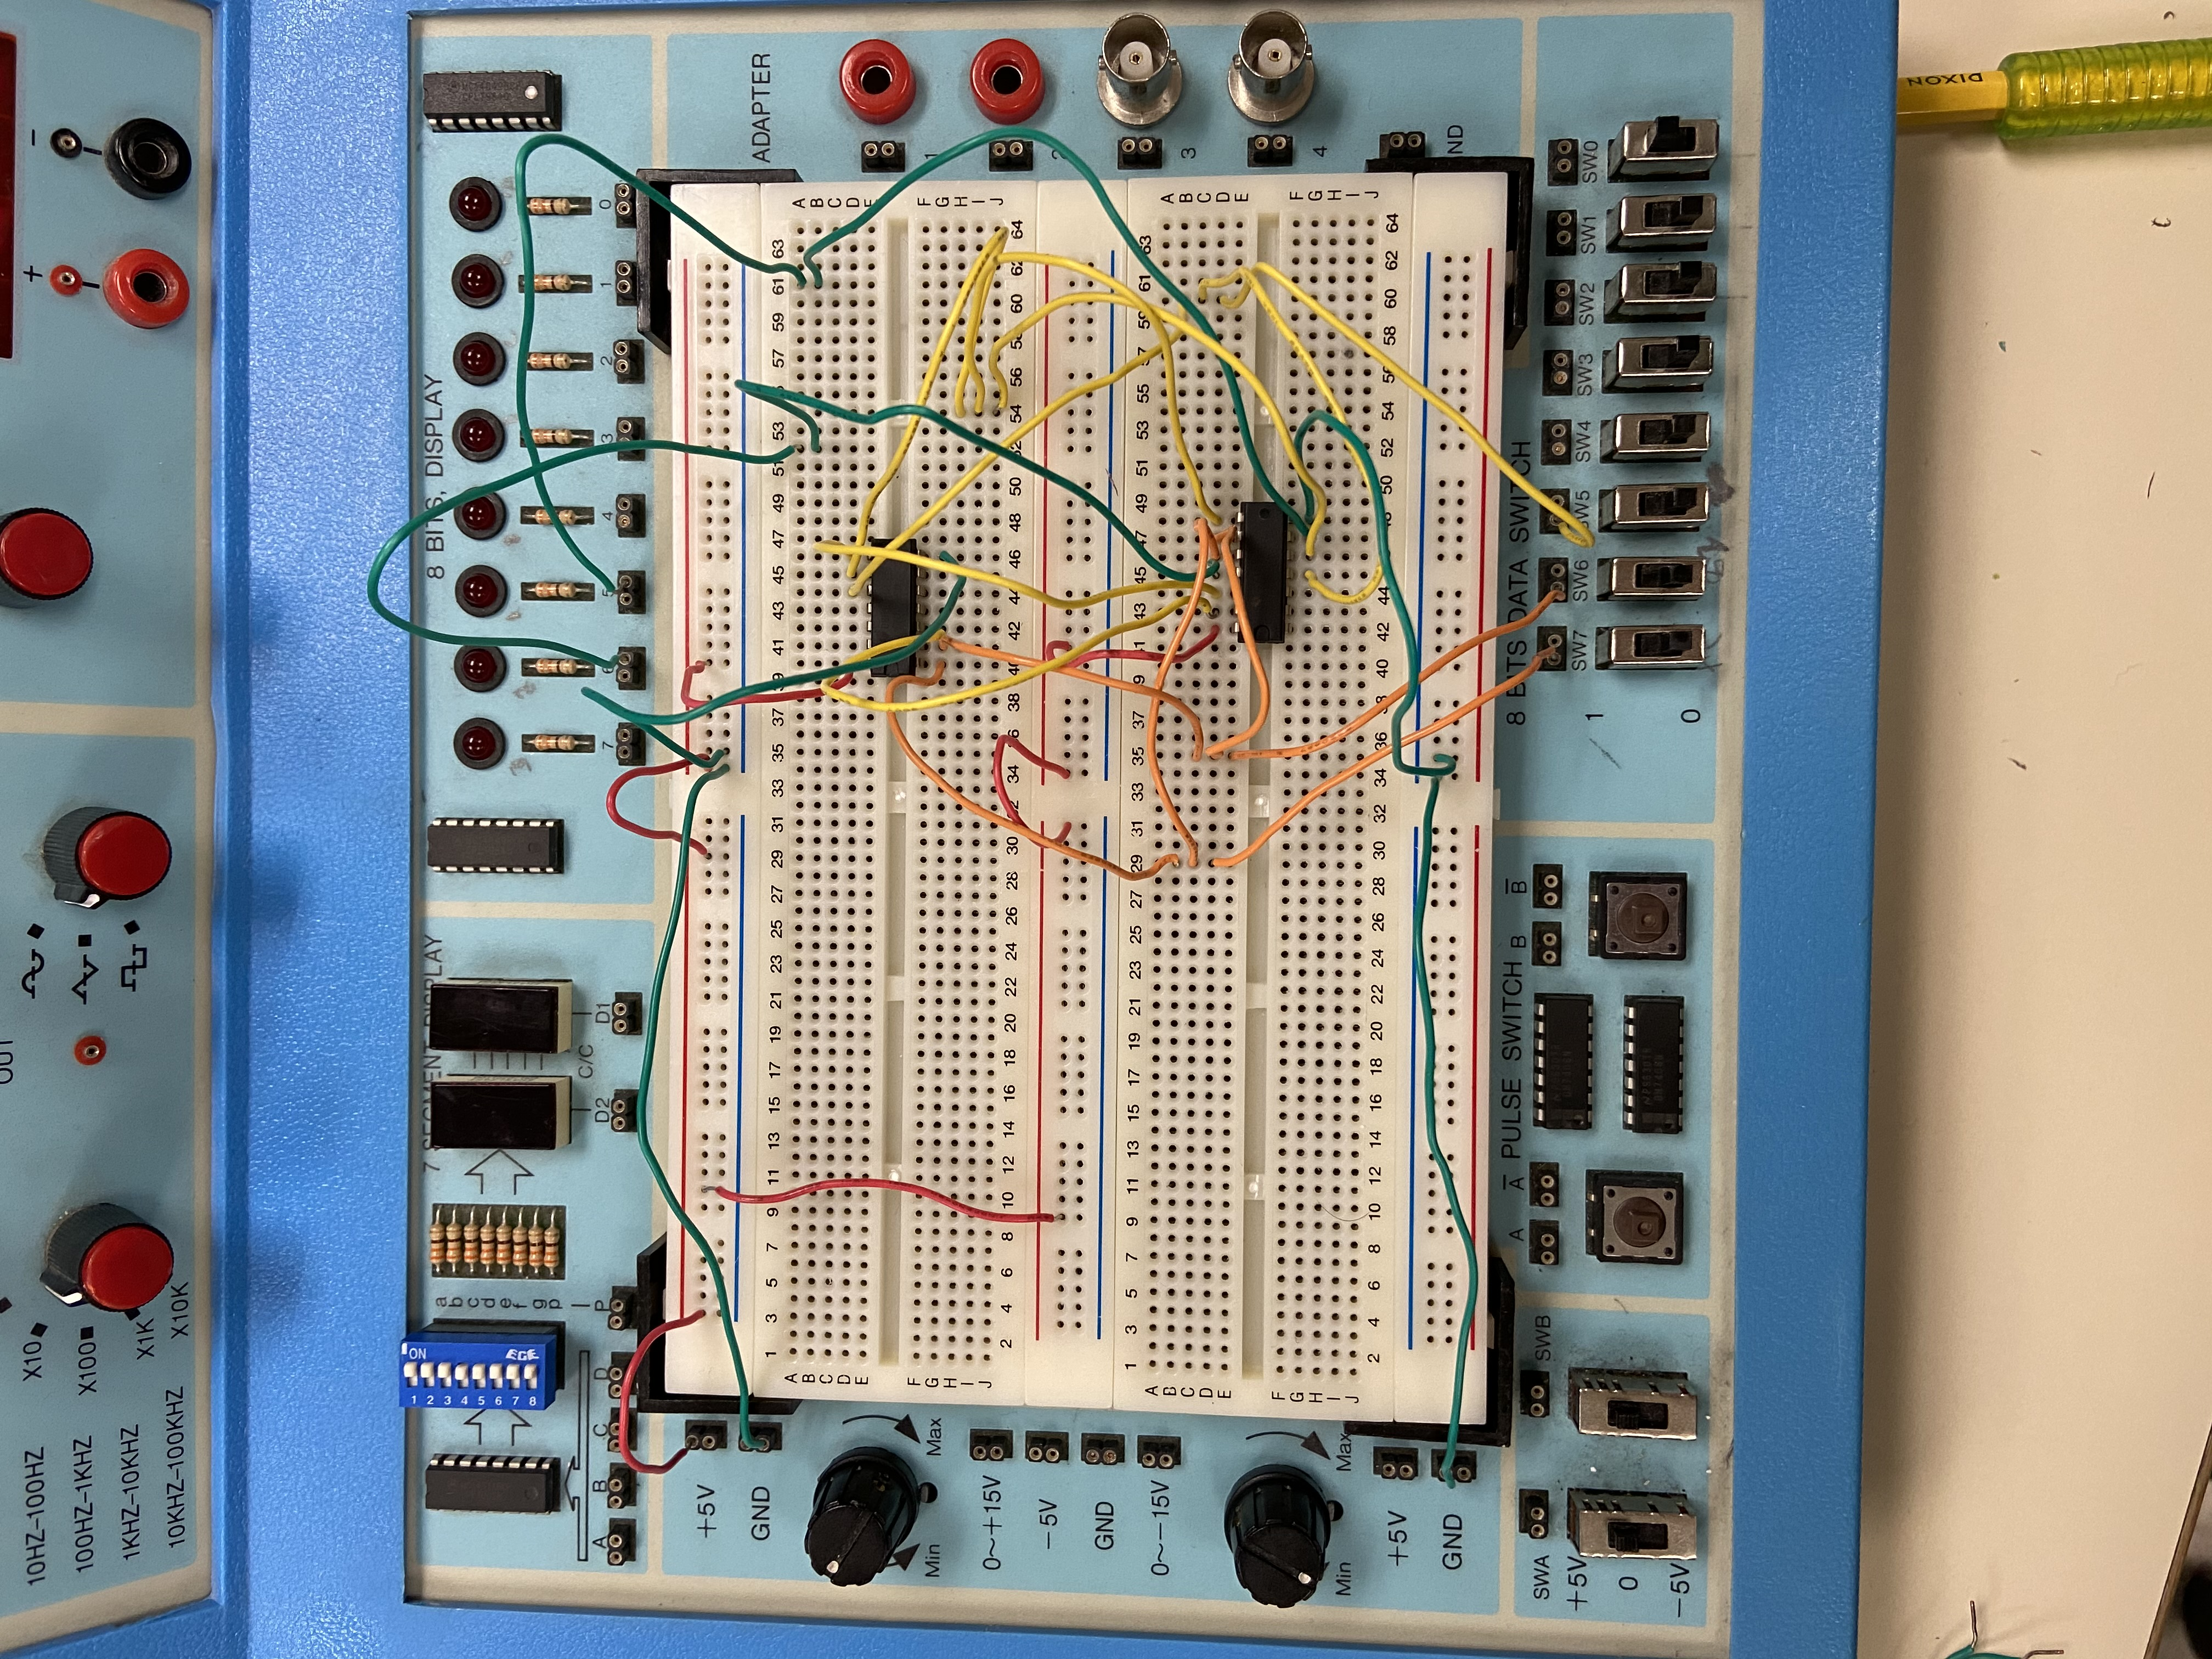
\includegraphics[width=0.75\textwidth, angle = 270]{Full Adder}
	\caption{This is the Full Adder.}
	\label{fig:original_logo}			% label must be after caption
\end{figure}

\begin{figure}[ht]\centering
	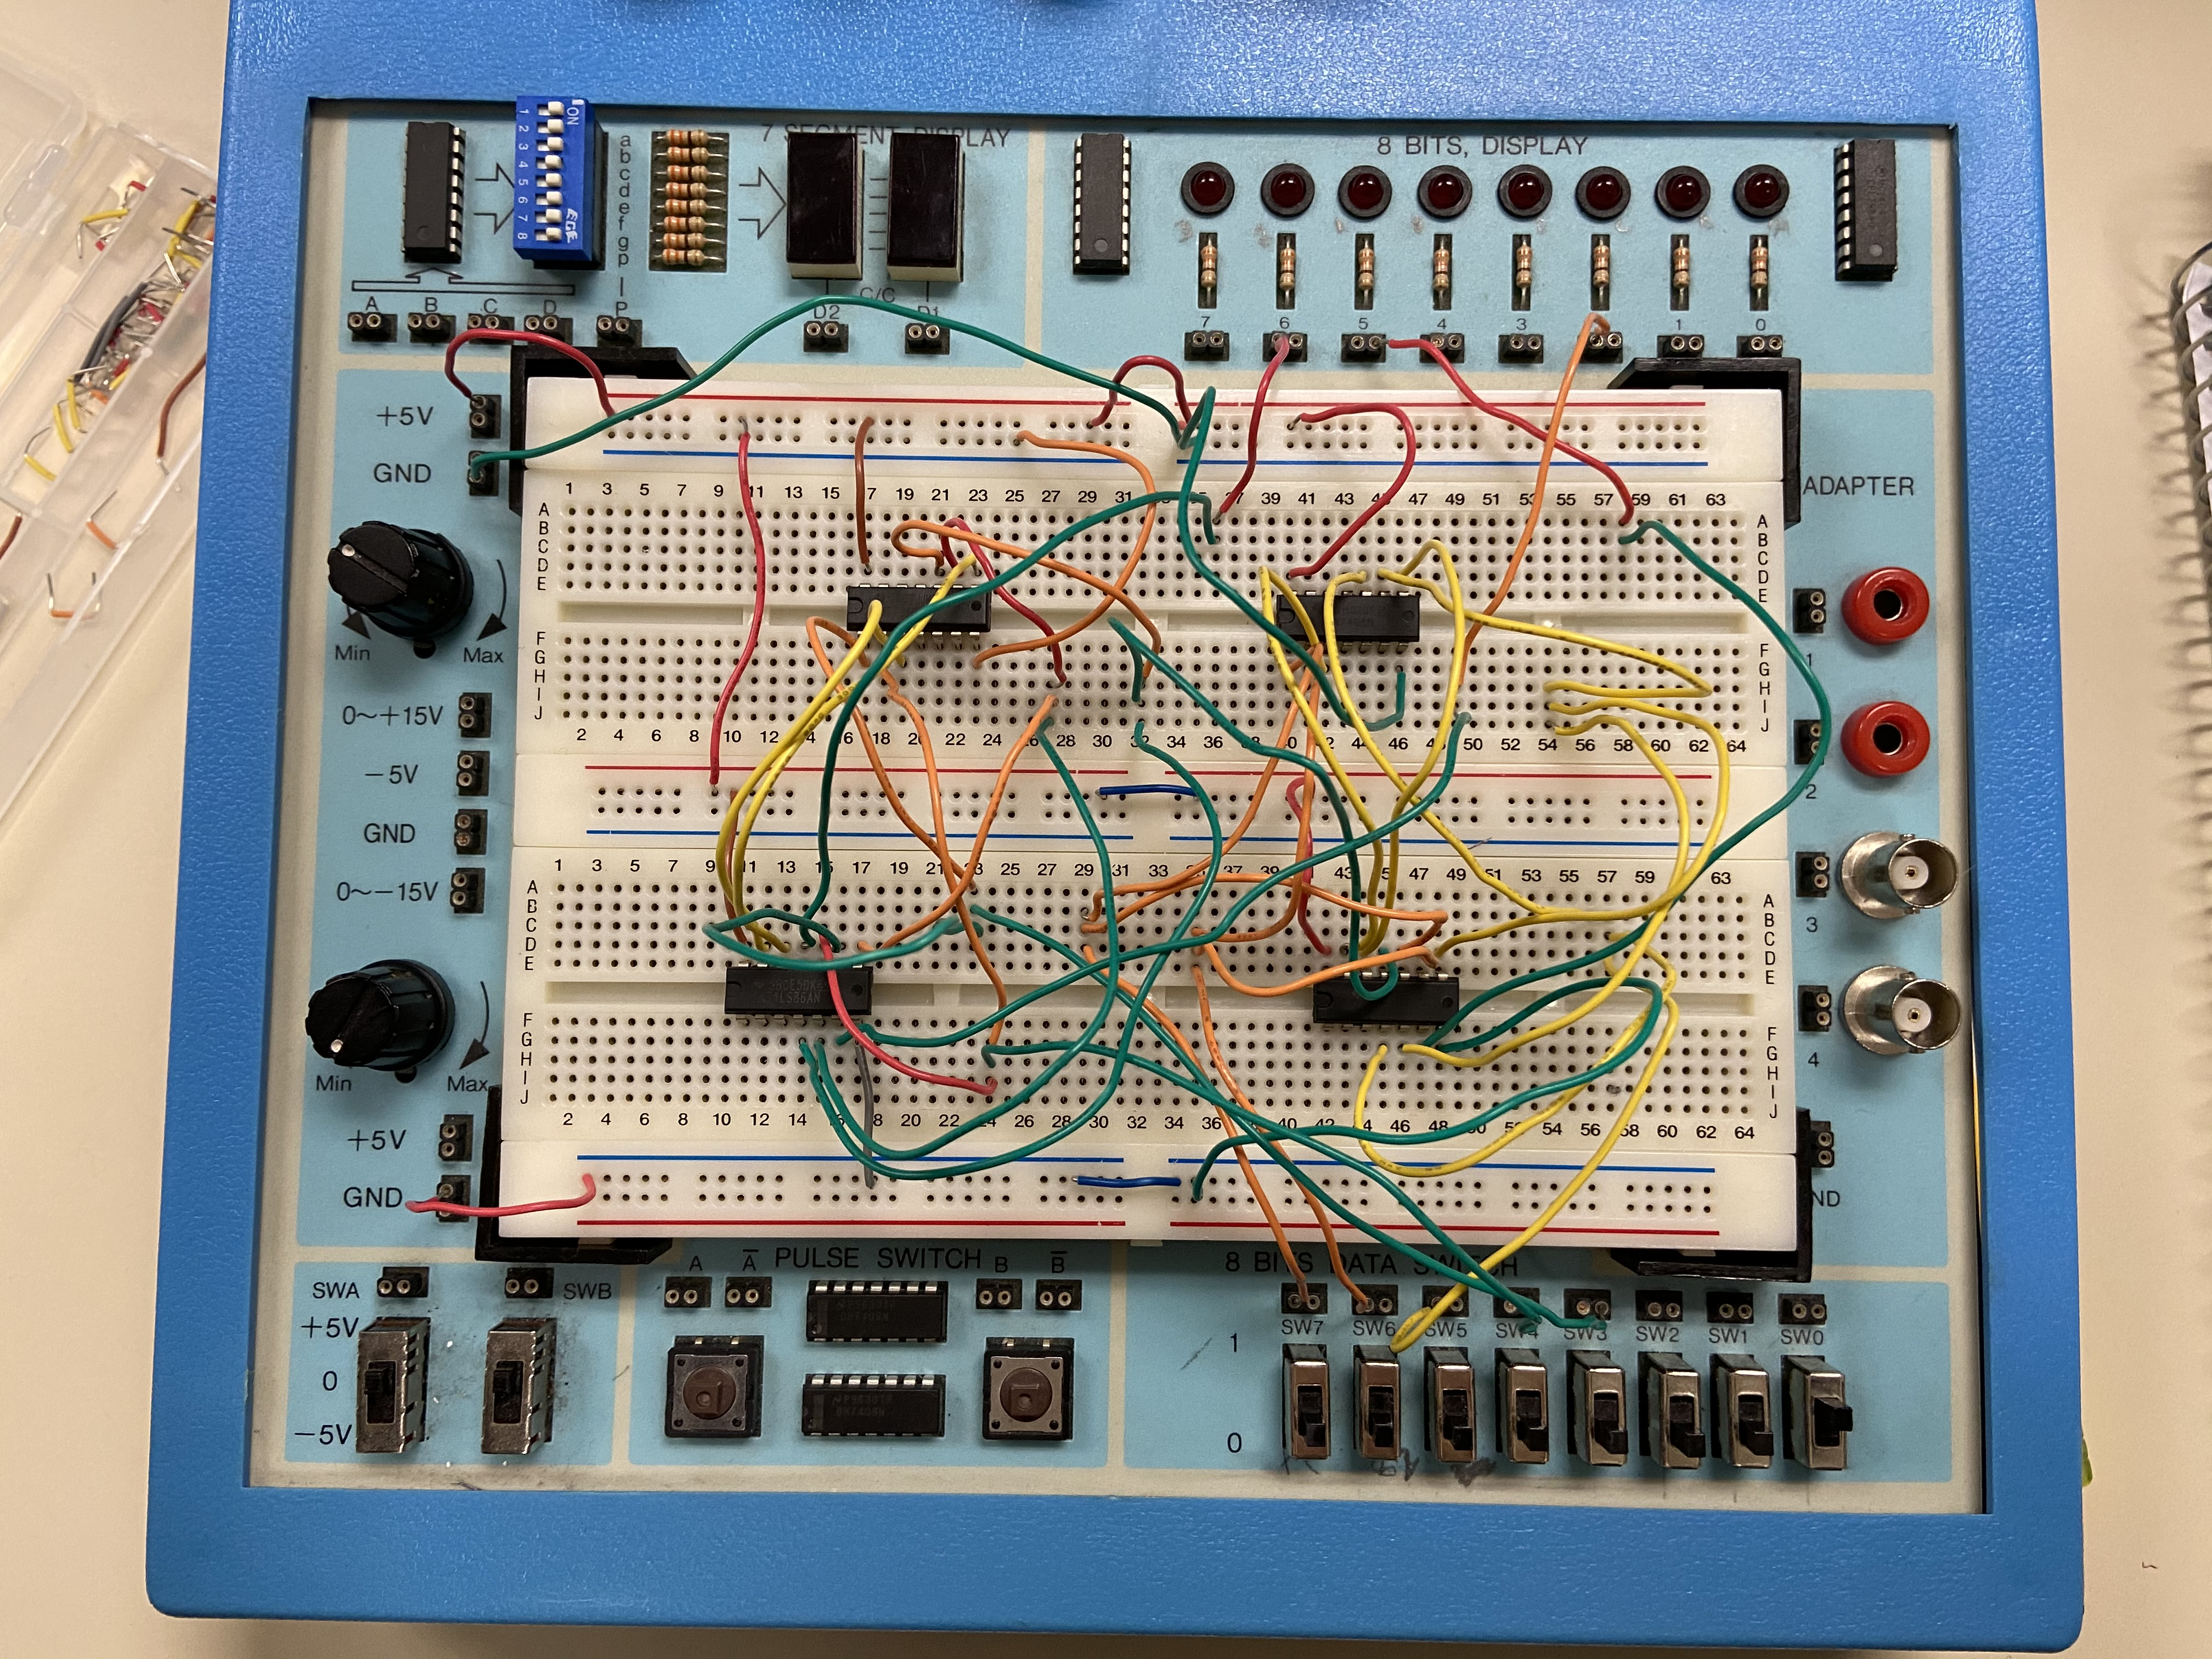
\includegraphics[width=0.75\textwidth]{2-bit Adder}
	\caption{This is the 2-bit Adder.}
	\label{fig:original_logo}			% label must be after caption
\end{figure}



\end{document}
